\section{Label-Noise Stress Test}

The contamination model in Appendix B predicts that rare high-loss samples can dominate EF-EWC because their loss-gradient scales enter the empirical Fisher directly. Controlled label noise instantiates this mechanism: corrupted labels create atypical high-loss training samples, while clean task-aware test sets measure whether the stored preservation matrix still protects the original classification structure. We therefore add uniform label noise to the CIFAR-100 training data in FACIL and report final average task-aware accuracy. IEWC degrades much more slowly than EF-EWC as the label-noise rate increases.

\begin{table}[t]
\centering
\begin{tabular}{lrrr}
\toprule
Method & $p=0$ & $p=0.1$ & $p=0.25$ \\
\midrule
EF-EWC & 0.5617 $\pm$ 0.0062 & 0.5132 $\pm$ 0.0112 & 0.2773 $\pm$ 0.0320 \\
EWC-DR & 0.5932 $\pm$ 0.0296 & 0.5310 $\pm$ 0.0226 & 0.4598 $\pm$ 0.0095 \\
IEWC & 0.5978 $\pm$ 0.0260 & 0.5642 $\pm$ 0.0215 & 0.5322 $\pm$ 0.0239 \\
\bottomrule
\end{tabular}
\end{table}

To connect this performance effect to the matrix-level prediction of the contamination model, we also record the largest stored diagonal entries of the EF and IEWC matrices on the same CIFAR-100 prefix protocol. These are not low-rank approximations. For diagonal matrices, the relevant stability object is the high-importance coordinate tail, so the table uses all 512 exported entries per matrix and reports the stored-tail mass ratio, the normalized stored-tail profile change, and the log-scale RMSE of the sorted entries. EF-EWC changes much more under contamination than IEWC on the log-scale metric.

\begin{table}[t]
\centering
\begin{tabular}{lrrrrr}
\toprule
Method & Noise & Entries & Stored-tail mass ratio & Stored-tail profile L1 & Stored-tail log-scale RMSE \\
\midrule
EF-EWC & 0.1 & 512 & 0.0288 & 0.2610 & 1.4660 \\
EF-EWC & 0.25 & 512 & 0.0244 & 0.2737 & 1.5337 \\
IEWC & 0.1 & 512 & 1.0833 & 0.0350 & 0.0350 \\
IEWC & 0.25 & 512 & 1.1003 & 0.0154 & 0.0415 \\
\bottomrule
\end{tabular}
\end{table}

\begin{figure}[H]
\centering
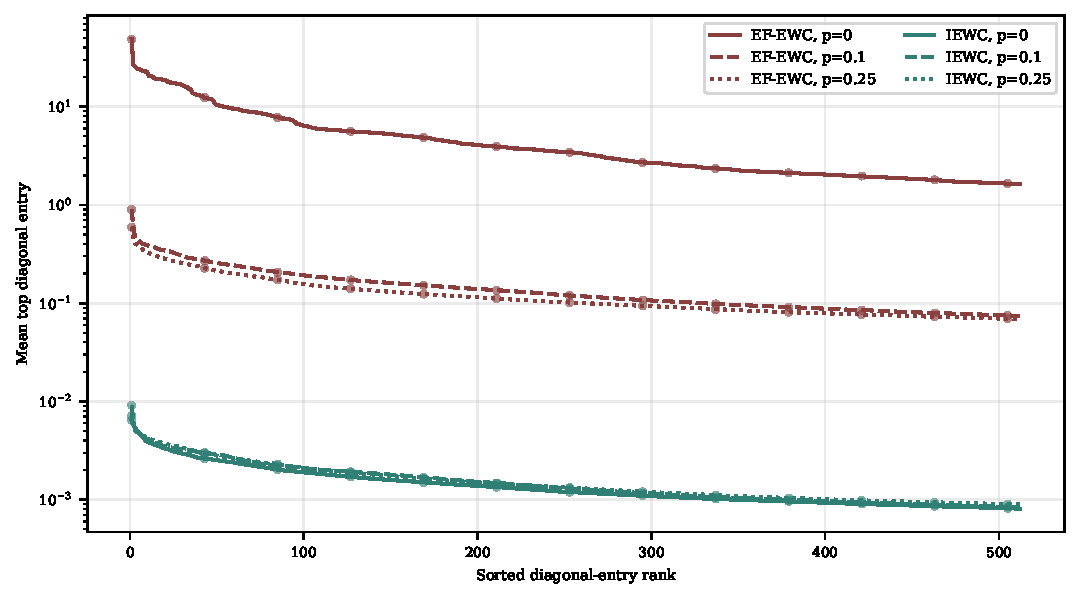
\includegraphics[width=0.54\linewidth]{figures/contamination_diagonal_spectra.pdf}
\caption[Label-noise diagonal spectra]{Label-noise diagonal spectra. The plot visualizes the high-importance coordinate tail underlying the matrix-level comparison above; EF-EWC changes much more under contamination than IEWC on the log scale.}
\label{fig:contamination-diagonal-spectra}
\end{figure}
